\documentclass{report}

\usepackage{amsmath} % provides numberwithin (and lots more)
\usepackage{graphicx}
\usepackage[backend=bibtex]{biblatex}
\bibliography{qfrmTechnicalQuestionsDev}


\newtheorem{problem}{}
\numberwithin{problem}{chapter} % important bit
\let\oldroblem\problem
\renewcommand{\problem}{\oldroblem\normalfont}
\newcommand{\ds}{\displaystyle}

\begin{document}

\begin{titlepage}
\begin{center}
 {\huge\bfseries Math 573\\ Lecture Notes\\}
 % ----------------------------------------------------------------
 \vspace{1.5cm}
% {\bfseries Instructor: Sergey Nadtochiy}\\[5pt]
% pbenson@umich.edu\\[14pt]
  % ----------------------------------------------------------------
 \vspace{10cm}
 % ----------------------------------------------------------------

\includegraphics{QFRM_rgb}\\[5pt]
{Department of Mathematics}\\[5pt]
{530 Church Street}\\[5pt]
{Ann Arbor, MI 48109-1043,
 USA}\\
 \vfill

\end{center}
\end{titlepage}

%----------------------
% review
%----------------------
\chapter{Introduction}

\section{What the course covers}
The course is divided broadly into three sections:
\begin{enumerate}  
\item Arbitrage pricing and hedging 
\item Optimal investment
\item Risk measurement
\end{enumerate}
Examples of each follow. Don't worry if the examples are unfamiliar at this time. They serve to indicate where we are headed. 

\subsection{Arbitrage Pricing and Hedging}
Let $C(K) \equiv$ the price of a European call option struck at $K$. Suppose that there are call options with strike prices of 1, 2, and 3 as depicted. 

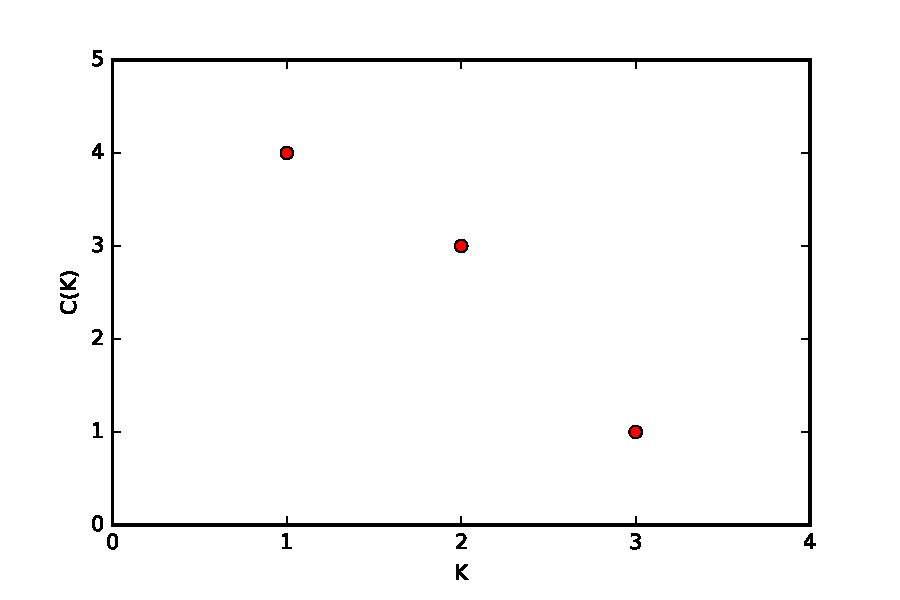
\includegraphics[width=8cm]{call-arb.pdf}

Is arbitrage possible? We note that if, for example, we buy 1 call struck at 1, sell 2 calls struck at 2, and buy 2 struck at 3, we will have spent 4 - 2(3) + 2(1) = 0. But as we will see, this portfolio will never have negative value, and can have positive value at expiry. So there is arbitrage.

\subsection{Optimal Investment}
Consider stocks that have been selected from an index. We wish to construct a portfolio from these stocks. A commonly used approach is to weight each stock $i$ according to its relative market cap:
\begin{eqnarray*}
w_i = \frac{\mbox{market cap of }i}{\mbox{combined market cap of stocks}}
\end{eqnarray*}
Why do portfolio managers use this weighting scheme? The answer is that according to CAPM (Capital Asset Pricing Model) theory, this portfolio gives the best return relative to the risk of the portfolio.

\subsection{Risk Measurement}
How can we measure the risk of the portfolio? ...

\pagebreak
%\section{Markets, Assets, Trades, and Derivatives}
\section{Markets, Assets, Trades, and Derivatives}

%\subsection{Markets}
\subsection{Markets}
We distinguish two types of markets:
\begin{enumerate}  
\item exchanges, where prices are well-known
\item OTC (over-the-counter), where prices are not necessarily observed
\end{enumerate}
How do we price an OTC security?

%\subsection{Assets}
\subsection{Assets}
We will consider the following types of assets:
\begin{enumerate}  
\item stocks (equities)
\item bonds (fixed income securities). For our purposes, we will assume these are risk-free (i.e. no credit risk, meaning there is no chance of default).
\item commodities and currencies
\item derivatives of the above
\end{enumerate}

\subsection{Trades}
A  {\it contract} is an agreement to exchange asset flows. 

A {\it trade} is the act of entering into a contract.

\end{document}
